% 402Pilot: An x402 Decision Layer for Autonomous Agent Micropayments
%
% Compiles out-of-the-box with article + geometry as a stub layout.
% Swap to the venue's style file (NeurIPS / ICML / ICLR / AAAI) before
% submission — see paper/README.md for instructions.

\documentclass{article}

% ---------------------------------------------------------------------
% Stub preamble (works without venue .sty). Replace as needed.
% ---------------------------------------------------------------------
\usepackage[utf8]{inputenc}
\usepackage[T1]{fontenc}
\usepackage[margin=1in]{geometry}    % stub layout; venue .sty supersedes
\usepackage{microtype}
\usepackage{hyperref}
\usepackage{url}
\usepackage{booktabs}
\usepackage{amsmath, amsfonts, amssymb}
\usepackage{nicefrac}
\usepackage{xcolor}
\usepackage{graphicx}
\usepackage{algorithm}
\usepackage[noend]{algpseudocode}

% ---------------------------------------------------------------------
% Notation macros — mirror logs/notation.md §10. Keep in sync.
% ---------------------------------------------------------------------
\newcommand{\nrm}{\mathrm{norm}}
\newcommand{\lamn}{\lambda_{\nrm}}
\newcommand{\bex}{\mathrm{burn\_excess}}
\newcommand{\padct}{PA\nobreakdash-DCT}
\newcommand{\rt}{r_t}
\newcommand{\ut}{u_t}
\newcommand{\ctilde}{\tilde c_t}
\newcommand{\thetaq}[2]{\theta_q^{#1,#2}}
\newcommand{\thetac}[2]{\theta_c^{#1,#2}}
\newcommand{\Sigmaq}[2]{\Sigma_q^{#1,#2}}
\newcommand{\Sigmac}[2]{\Sigma_c^{#1,#2}}
\newcommand{\hatu}[2]{\hat u^{#1,#2}}
\newcommand{\hatc}[2]{\hat c^{#1,#2}}
\newcommand{\Reg}{\mathrm{Regret}}
\newcommand{\AdaptT}{\tau_{\mathrm{adapt}}}

% ---------------------------------------------------------------------
% Title block
% ---------------------------------------------------------------------
\title{402Pilot: An x402 Decision Layer for\\Autonomous Agent Micropayments}
\author{
  Anonymous Author(s)\\
  Affiliation\\
  \texttt{email}
}
\date{}

\begin{document}
\maketitle

\begin{abstract}
A new family of programmable payment protocols (x402, AP2, A2A--x402, A402) lets autonomous agents pay for online services at machine speed, but supplies no algorithm for the buyer's first decision: which provider to pay. We formalize this gap as \emph{agent-native bandits}---budget-aware, non-stationary, contextual decision-making over heterogeneous paid providers, where the bandit is the autonomous buyer itself rather than a human-operated routing service. We propose \emph{402Pilot}, a protocol-agnostic decision layer with stable interfaces between agent decision-making and payment execution, and \emph{PA-DCT} (Payment-Aware Discounted Contextual Thompson sampling), the policy that drives it. PA-DCT maintains discounted dual Gaussian posteriors over both quality and cost per (provider, task-type) bucket, treating cost as a learned signal rather than a known scalar so that price shocks are detected the same way quality shocks are. We construct \emph{402Pilot-Bench}, a reproducible replay benchmark of $824$ tasks across coding, multi-hop QA, and web search; five heterogeneous LLM providers including adversarial and flaky variants at the same price tier; three calibrated market scenarios (stationary, mid-tier outage, premium price promotion); and $30$ seeds $\times$ $10{,}000$ rounds per cell, totaling $20{,}575$ pre-generated frozen LLM responses. PA-DCT outperforms five baselines under both non-stationary scenarios with paired-bootstrap significance at $p<10^{-3}$, while paying a small honest exploration cost in the stationary baseline. A four-component ablation isolates which classical bandit ingredients transfer to the agent-native regime, and shows that no single metric reveals all four; we recommend a multi-metric evaluation framework for future work in this setting.

\end{abstract}

\section{Introduction}
\label{sec:intro}

% TODO: ~1.25 pages (paper_outline.md §1).
%
% Beats:
% 1. Agents are becoming economic actors: wallets, per-call APIs,
%    micropayments. The protocol stack (x402, A402, ...) handles execution.
% 2. But execution is not decision. An agent with a $50 wallet and five
%    providers — including an adversarial one and a flaky one — needs a
%    selection policy.
% 3. Existing solutions miss the regime: budget guardrails are rule-based,
%    LLM routing is offline cost optimization on one platform.
% 4. The gap: an online, budget-aware, non-stationary policy that
%    distinguishes providers from reward feedback alone.
% 5. Motivating example (boxed inset): mixed task workload, P-mid /
%    P-adv / P-flaky share cost tier and base model — only outcomes
%    distinguish them. Static rules cannot. PA-DCT can.
% 6. Coin the term \emph{agent-native bandits}: bandit settings where the
%    operator IS the agent, not a human ML team.
% 7. Contributions C1-C5 (see logs/paper_design_decisions.md §11.4).

\section{Related Work}
\label{sec:related-work}

Four threads of prior work bear on 402Pilot.

\paragraph{Agent payment protocols.}
x402~\cite{coinbase2025x402v2}, A402~\cite{a402}, and a recent {SoK} on agent payments~\cite{sok2026agentpayments} define the protocol stack for machine-to-machine micropayments: identity, settlement, capability discovery. The x402 V2 specification explicitly defers provider selection to the buyer based on ``historical outcomes.'' None of this work proposes a decision algorithm. 402Pilot fills that gap: it answers \emph{which} provider to pay, while protocol primitives remain responsible for \emph{how} the payment executes.

\paragraph{Classical bandit components.}
\padct{} inherits from three lines of bandit research. Budgeted Thompson sampling~\cite{xia2015bts} treats finite spend as a constraint, but assumes stationary scalar costs and no context. Discounted TS over sufficient statistics~\cite{qi2023dsts} handles non-stationary rewards through exponential forgetting, but ignores budget and context. Contextual Thompson sampling for linear payoffs~\cite{agrawal2013contextualts} is the canonical Bayesian recipe we adapt to a bucketed-Gaussian setting; LinUCB~\cite{li2010linucb} is its frequentist counterpart. The bandits-with-knapsacks formalism~\cite{badanidiyuru2018bandits} supplies the standard budget framing. To our knowledge, no prior work combines budget-aware, discounted, and contextual Thompson sampling into a single decision rule with separate posteriors over both quality and cost.

\paragraph{LLM cost-aware routing.}
Several recent systems address the quality--cost tradeoff in LLM cascading. FrugalGPT~\cite{chen2023frugalgpt} introduced the cost-aware cascade with a fixed escalation rule. RouteLLM~\cite{ong2024routellm}, Hybrid LLM~\cite{ding2024hybridllm}, MixLLM~\cite{mixllm2024}, and AutoMix~\cite{madaan2024automix} train classifiers or self-verifiers to route between two or more LLMs offline. They share \padct{}'s motivation but differ structurally: cost is a static rate card, no payment protocol enters the decision loop, and evaluation is on offline test sets rather than non-stationary online markets. Our BudgetRule baseline is essentially a FrugalGPT-style fixed threshold; \padct{} outperforms it under S2 outage and S3 promotional repricing.

\paragraph{The most adjacent paper.}
A concurrent {AAMAS} 2026 paper on truthful reverse auctions for adaptive LLM selection~\cite{aamas2026reverseauction} also applies a contextual MAB to online provider choice. We share the algorithmic family but differ structurally. \emph{Mechanism}: \cite{aamas2026reverseauction} runs a reverse auction in which providers submit bids; we operate against x402's quote-and-pay flow with posted prices. \emph{Framing}: their object of study is incentive compatibility for strategic providers; ours is a decision layer with non-strategic providers and a wallet that drains. \emph{Benchmark}: their evaluation does not target the non-stationary scenarios (outage, repricing) we use. The two contributions are complementary.

\section{Problem Formulation}
\label{sec:problem}

\paragraph{Quote--pay--observe setting.}
We consider a single autonomous buyer with initial wallet budget $B$ that repeatedly chooses among $K$ payable service providers over rounds $t \in \{0,\ldots,T-1\}$. At the start of round $t$, the buyer observes a task context $\mathbf{x}_t \in \mathcal{X}$ and the wallet state $B_t$. A programmable payment interface exposes enough price information to determine which providers are affordable before payment; let $p_{a,t}$ denote the pre-payment quote for provider $a$, and define
\begin{equation}
\label{eq:affordable-set}
\mathcal{A}_t = \{a \in \{1,\ldots,K\}: p_{a,t} \leq B_t\}.
\end{equation}
The quote is available before selection; the realized charged cost $c_t$ is observed after the selected payment and is kept as the cost feedback signal across rounds. If $\mathcal{A}_t$ is empty, the run stops. Otherwise, the buyer selects one provider $a_t \in \mathcal{A}_t$, commits to the paid call through the protocol, and cannot observe the service outcome before paying.

\paragraph{Feedback and wallet dynamics.}
After the selected call completes, the buyer observes only the chosen provider's outcome:
\[
(q_t, c_t, f_t) \sim \mathcal{D}_{a_t,t}(\cdot \mid \mathbf{x}_t),
\]
where $q_t \in [0,1]$ is a task-level quality score, $c_t \in \mathbb{R}_{\geq 0}$ is the realized charged cost, and $f_t \in \{0,1\}$ marks timeout, parse failure, or another non-delivery event. Outcomes and realized charges for unchosen providers are not observed as samples; this is the bandit feedback that makes provider choice a learning problem rather than a full-information ranking problem. The wallet evolves deterministically as
\begin{equation}
\label{eq:wallet}
B_{t+1} = B_t - c_t, \qquad B_0 = B,
\end{equation}
and $\tau \leq T$ denotes the first round at which the horizon is reached or no provider is affordable.

\paragraph{Utility and objective.}
We separate intrinsic service delivery from payment pressure. Utility combines quality with a structural failure penalty:
\begin{equation}
\label{eq:utility}
\ut = q_t - \nu f_t.
\end{equation}
The penalty captures retry overhead, broken call chains, and downstream agent stalls that are not fully represented by setting $q_t=0$ on failure.

The payment-aware reward combines utility with normalized realized cost:
\begin{equation}
\label{eq:reward}
\ctilde = \mathrm{clip}(c_t/c_{\max},0,1), \qquad
\lamn = \frac{\lambda_t}{1+\lambda_t}, \qquad
\rt = (1-\lamn)\ut - \lamn\ctilde .
\end{equation}
Here $c_{\max}$ is a fixed cost normalizer and $\lambda_t \geq 0$ is the wallet-pressure multiplier defined below. The bounded weight $\lamn \in [0,1]$ keeps utility and cost comparable across wallet states while preserving the sign of failures. A policy $\pi$ aims to maximize the expected cumulative payment-aware reward
\begin{equation}
\label{eq:objective}
J(\pi) = \mathbb{E}_{\pi}\!\left[\sum_{t=0}^{\tau-1} \rt \right],
\end{equation}
subject to the affordability constraint in Eq.~\eqref{eq:affordable-set}. In PA-DCT, beliefs are updated from the two observed channels $(\ut,c_t)$ rather than from the scalar $\rt$: $\ut$ tracks provider quality, $c_t$ tracks realized payment cost, and $\rt$ defines the decision/evaluation objective.

\paragraph{Budget pressure.}
The wallet-pressure multiplier is a deterministic function of cumulative spend. For $t>0$, define the realized burn rate as the fraction of the wallet spent per elapsed round,
\begin{equation}
\label{eq:burn-rate}
\mathrm{actual\_burn\_rate}_t = \frac{(B-B_t)/B}{t},
\qquad
\mathrm{target\_rate} = \frac{1}{T}.
\end{equation}
The normalized burn deviation is
\begin{equation}
\label{eq:lambda}
\bex_t =
\frac{\mathrm{actual\_burn\_rate}_t-\mathrm{target\_rate}}
{\mathrm{target\_rate}},
\qquad
\lambda_t =
\begin{cases}
1, & t=0,\\
\exp(\alpha \bex_t), & t>0,
\end{cases}
\end{equation}
with sharpness parameter $\alpha \geq 0$. Thus $\lamn=0.5$ when the buyer is exactly on the linear burn plan, decreases when the buyer is under-spending, and increases toward cost-dominated decisions when the wallet is being spent too quickly.

\paragraph{Non-stationarity and scope.}
Provider distributions $\mathcal{D}_{a,t}(\cdot \mid \mathbf{x})$ may change over time in utility, reliability, or realized cost. Change points are not announced to the policy. Tasks arrive from an exogenous workload stream, and providers are non-strategic posted-price endpoints: they expose quotes and deliver services rather than bidding strategically for allocation. Reverse auctions, multi-agent coordination, dispute resolution, and latency-aware routing are outside this formulation.

\paragraph{Why a contextual bandit.}
The only controlled action in a round is the provider choice $a_t$; the immediate feedback is the selected call's $(\ut,c_t)$, and the only persistent state affected by the action is deterministic wallet accounting. There is no delayed reward, within-round planning horizon, or latent transition model to learn. We therefore formulate agent-native payment decision-making as a contextual bandit with budget state and non-stationary feedback, rather than as a full reinforcement-learning problem.

\section{The 402Pilot Decision Layer}
\label{sec:layer}

402Pilot is a decision layer between an autonomous agent and a programmable payment protocol such as x402. The layer accepts a task and a wallet state, picks a provider, calls the protocol stack to settle the payment, and feeds the realized outcome back into a policy. It does not modify the protocol, never holds funds, and never crosses the settlement boundary. Figure~\ref{fig:architecture} sketches the per-round flow.

\begin{figure}[t]
\centering
\resizebox{\textwidth}{!}{%
\begin{tikzpicture}[
  font=\footnotesize,
  node distance=1.15cm and 1.0cm,
  block/.style={
    draw=black!55,
    rounded corners=2pt,
    align=center,
    minimum height=0.78cm,
    text width=2.15cm,
    inner sep=4pt,
    fill=white
  },
  pilotblock/.style={block, draw=blue!55!black, fill=blue!5},
  extblock/.style={block, draw=black!45, fill=black!7},
  payblock/.style={block, draw=black!45, fill=black!10, dashed},
  arrow/.style={-{Stealth[length=2.0mm]}, line width=0.45pt},
  feedback/.style={-{Stealth[length=2.0mm]}, line width=0.45pt, dashed},
  lab/.style={font=\scriptsize, fill=white, inner sep=1.5pt}
]

\node[extblock] (agent) {Agent\\planner};
\node[pilotblock, right=of agent] (ctx) {Context\\encoder\\$\mathbf{x}_t$};
\node[pilotblock, right=of ctx] (wallet) {Wallet /\\budget\\$\lambda_t,\mathcal{A}_t$};
\node[pilotblock, right=of wallet, text width=2.35cm] (select) {PA-DCT\\\texttt{policy.select}\\$a_t$};
\node[payblock, right=of select, text width=2.3cm] (x402) {Payment\\protocol stack\\(e.g., x402)};
\node[payblock, right=of x402] (provider) {Chosen\\provider\\$a_t$};
\node[extblock, below=1.1cm of x402, text width=2.35cm] (eval) {Outcome\\evaluator\\$q_t,c_t,f_t$};
\node[pilotblock, below=1.1cm of select, text width=2.45cm] (update) {Reward split +\\\texttt{policy.update}\\$u_t=q_t-\nu f_t$};

\begin{scope}[on background layer]
  \node[
    draw=blue!45!black,
    fill=blue!3,
    rounded corners=4pt,
    inner xsep=7pt,
    inner ysep=9pt,
    fit=(ctx) (wallet) (select) (update)
  ] (pilotbox) {};
  \node[
    draw=black!35,
    fill=black!4,
    rounded corners=4pt,
    dashed,
    inner xsep=7pt,
    inner ysep=9pt,
    fit=(x402) (provider)
  ] (paybox) {};
\end{scope}

\node[anchor=north west, font=\scriptsize\bfseries, text=blue!55!black]
  at ([xshift=2pt,yshift=-2pt]pilotbox.north west) {402Pilot decision layer};
\node[anchor=north west, font=\scriptsize\bfseries, text=black!55]
  at ([xshift=2pt,yshift=-2pt]paybox.north west) {delegated settlement / service execution};

\draw[arrow] (agent) -- node[lab, above] {(1) task} (ctx);
\draw[arrow] (ctx) -- node[lab, above] {(2) context} (wallet);
\draw[arrow] (wallet) -- node[lab, above] {(3) budget pressure + feasible arms} (select);
\draw[arrow] (select) -- node[lab, above] {(4) chosen arm} (x402);
\draw[arrow] (x402) -- node[lab, above] {(5) paid call} (provider);
\draw[arrow] (provider.south) |- node[lab, pos=0.28, right] {response} (eval.east);
\draw[arrow] (eval) -- node[lab, below] {(6) observed outcome} (update);
\draw[feedback] (update.north) -- node[lab, right] {(7) update Q/C posteriors} (select.south);
\draw[feedback] (update.west) -| node[lab, pos=0.25, below] {\texttt{record\_spend}$(c_t)$} (wallet.south);

\node[font=\scriptsize, align=center, text=black!65, below=0.18cm of update, text width=4.4cm]
  {Posteriors are updated with utility and realized cost; payment-aware reward is logged for accounting.};

\end{tikzpicture}%
}
\caption{The 402Pilot decision-layer architecture. Per round: (1) task arrives from the agent; (2) the context encoder produces $\mathbf{x}_t$; (3) the wallet exposes $\lambda_t$ and the affordable-arm set; (4) \texttt{policy.select} returns $a_t$; (5) the underlying payment protocol settles and calls the chosen provider (grayed: outside the layer); (6) the evaluator returns $(q_t, c_t, f_t)$; (7) \texttt{policy.update} incorporates the observation. Only steps 2--4 and 7 are inside 402Pilot; settlement is delegated unchanged.}
\label{fig:architecture}
\end{figure}

\paragraph{Two stable interfaces.}
A policy is any object exposing
\begin{align*}
&\mathtt{select}(\mathbf{x}_t,\, \mathcal{A}_t,\, \mathrm{wallet\_state}) \to a_t \in \mathcal{A}_t, \\
&\mathtt{update}(\mathbf{x}_t,\, a_t,\, \ut,\, c_t) \to \emptyset,
\end{align*}
where $\mathcal{A}_t \subseteq \{1, \ldots, K\}$ is the set of providers that fit in the remaining wallet at the current effective prices. Affordability is enforced by the wallet, not the policy: a policy never has to reason about hard budget constraints, only about picking well from a feasible set. The two methods are the only points of contact with the rest of the stack; everything else (priors, posteriors, internal state) is private to the policy.

\paragraph{Update signal: utility, not payment-aware reward.}
A subtle but load-bearing commitment: the layer feeds \emph{utility} $\ut$ to \texttt{policy.update}, not the payment-aware reward $\rt$. This decoupling lets the posterior track \emph{intrinsic provider quality} independently of decision-time budget pressure. If we instead updated on $\rt$, beliefs about a provider would shift purely because the wallet drained, defeating the purpose of having a posterior. Concretely: the same provider should not look worse to the policy late in a budget-tight run than it did early in the run when the wallet was full. Decision-time budget pressure enters only inside \texttt{select}, through $\lamn$, never inside \texttt{update}.

\paragraph{Pluggability across policies and protocols.}
On the policy side, every comparator we evaluate (\S\ref{sec:eval-comparators})---Random, three Always-X variants, BudgetRule, and PA-DCT itself---implements the same two-method interface. New algorithms drop in without touching the rest of the stack. On the protocol side, the layer is agnostic to which programmable payment substrate sits below: today we instantiate above x402~\citep{coinbase2025x402v2}, but the same interfaces apply to AP2~\citep{google2025ap2}, A2A--x402~\citep{a2ax402}, A402~\citep{a402}, or any future quote-and-pay protocol. The protocol stack provides addressing, settlement, and audit trails; 402Pilot provides the decision policy.

\paragraph{What the layer does \emph{not} do.}
Five concerns are explicitly out of scope and are addressed in \S\ref{sec:discuss}:
on-chain settlement (the protocol's job);
capability discovery (handled by x402 V2's Discovery extension or equivalent registries);
production observability (operator dashboards, alerting);
multi-agent coordination (we operate at single-agent scope: one wallet, one policy, one workload stream);
and online safeguards such as drift detection or trust scoring (future work; we discuss directions in \S\ref{sec:discuss}).

\paragraph{What the layer assumes.}
402Pilot makes three assumptions about the surrounding stack. First, the protocol can quote a price for a paid call before the call is made, so the wallet can compute affordability and the policy can include cost in its decision rule. Second, outcomes are observable and scoreable shortly after the call, so the policy can update before the next round (we make this concrete in our benchmark via deterministic per-task evaluators or cached LLM-as-judge scores). Third, providers are non-strategic in the protocol-mechanism sense: they post prices and deliver services rather than playing auction games over bids. All three assumptions hold for x402 V2 and its current peers. Relaxing the third---strategic providers---is the regime studied by recent mechanism-design work~\citep{aamas2026reverseauction}; 402Pilot is complementary to that line, not a substitute.

\paragraph{Implementation footprint.}
The reference implementation is a Python package (\texttt{pilot402}) of approximately [/cc TODO line count] lines, with the policy interface, the wallet, the context encoder, the reward calculator, and the per-seed runtime loop as separate modules; any one of them can be swapped without touching the others. The full benchmark harness, including pre-generated dataset and scenario sweeps, runs end-to-end in approximately [/cc TODO wall-clock estimate; current main sweep takes \~X hours on a laptop] and is released alongside this paper.

\section{Method: PA-DCT}
\label{sec:method}

PA-DCT is an instance of contextual Thompson sampling adapted to the agent-native regime (\S\ref{sec:intro}). Each (arm, task-type-bucket) cell maintains \emph{two} independent Gaussian posteriors---one over utility, one over cost---both tracked through discounted sufficient statistics. At decision time, the policy samples both posteriors and ranks affordable arms by a budget-pressure-weighted score; on receipt of the realized outcome, only the chosen cell's posteriors are updated, after a global discount sweep over every cell.

\subsection{Dual Gaussian posteriors}
\label{sec:method-posteriors}

For each arm $a \in \{1,\ldots,K\}$ and bucket $k \in \{1,\ldots,K_b\}$ (where $K_b$ is the number of context buckets, default $4$, one per task type), we maintain two posteriors:
\begin{itemize}
\item \textbf{Q-posterior}, tracking the per-arm utility $\ut = q_t - \nu f_t$. Conjugate Normal-Normal with prior $\mathcal{N}(\mu_{0,q}, \sigma^2_{0,q})$ and likelihood variance $\sigma^2_q$.
\item \textbf{C-posterior}, tracking the per-arm raw cost $c_t$. Same Normal-Normal form, with prior $\mathcal{N}(\bar c_a, \sigma^2_{0,c})$ where $\bar c_a$ is the spec base price for arm $a$, and likelihood variance $\sigma^2_c$.
\end{itemize}

Each cell carries the standard discounted sufficient statistics $n^{a,k}_t \in \mathbb{R}_{\geq 0}$ (effective sample count) and $S^{a,k}_t \in \mathbb{R}$ (weighted sum of observations), with the analogous pair for the cost posterior. Posterior parameters follow the closed-form Normal-Normal expressions, e.g.\ for Q:
\begin{equation}
\label{eq:posterior-q}
\Sigmaq{a}{k} = \left(\frac{1}{\sigma^2_{0,q}} + \frac{n^{a,k}_t}{\sigma^2_q}\right)^{-1}, \qquad
\thetaq{a}{k} = \Sigmaq{a}{k} \left(\frac{\mu_{0,q}}{\sigma^2_{0,q}} + \frac{S^{a,k}_t}{\sigma^2_q}\right).
\end{equation}
The C-posterior uses the analogous form with $(\thetac{a}{k}, \Sigmac{a}{k})$, $\bar c_a$ in place of $\mu_{0,q}$, $\sigma^2_c$ in place of $\sigma^2_q$, and a separate pair of sufficient statistics over realized costs.

\paragraph{Why a learned cost posterior.}
In stationary settings with known prices, a fixed scalar $\bar c_a$ would suffice for cost. The agent-native regime drops both assumptions: prices can change mid-run (S3 in our benchmark), and the agent only sees prices through quoted observations from the market. Treating cost as a Gaussian posterior over realized $c_t$ lets the policy detect price shocks the same way the Q-posterior detects quality shocks---through the effective sample count $n^{a,k}_t$ and the discount that reweights stale observations. We demonstrate empirically (\S\ref{sec:eval-ablations}) that disabling this and pinning cost to $\bar c_a$ collapses adaptation to S3.

\subsection{Discounted sufficient statistics}
\label{sec:method-discount}

We apply a multiplicative discount $\gamma \in (0, 1]$ to every cell's $n$ and $S$ at the start of each round, before any new observation arrives:
\begin{equation}
n^{a,k}_t = \gamma \cdot n^{a,k}_{t-1}, \qquad
S^{a,k}_t = \gamma \cdot S^{a,k}_{t-1}.
\end{equation}
After the round's chosen arm produces an observation, only its bucket increments:
\begin{equation}
n^{a_t, k_t}_t \mathrel{+}= 1, \quad
S^{a_t, k_t}_t \mathrel{+}= \ut\,\,(\text{Q-posterior}), \quad
{S_c}^{a_t, k_t}_t \mathrel{+}= c_t\,\,(\text{C-posterior}).
\end{equation}
Discounting applies regardless of whether a cell was pulled this round---non-stationarity is wall-clock, not pull-conditional. We use $\gamma = 0.999$ for both posteriors (effective half-life $\approx 693$ rounds), chosen to react cleanly within the shock windows we evaluate (S2 covers $2{,}500$ rounds, S3 has $9{,}000$ post-shock rounds) without forgetting the stationary baseline too quickly. Sensitivity to $\gamma$ is in [/cc TODO sensitivity appendix].

\subsection{Decision rule}
\label{sec:method-decision}

At each round, the wallet exposes $\lambda_t$ and the affordable set $\mathcal{A}_t$. The policy reads $\lamn$ from the wallet, samples both posteriors per affordable arm, and ranks them:
\begin{equation}
\label{eq:padct-sample}
\hatu{a}{k_t} \sim \mathcal{N}\!\big(\thetaq{a}{k_t},\, \Sigmaq{a}{k_t}\big), \qquad
\hatc{a}{k_t} \sim \mathcal{N}\!\big(\thetac{a}{k_t},\, \Sigmac{a}{k_t}\big),
\end{equation}
\begin{equation}
\label{eq:padct-score}
\tilde{\hat c}^{a,k_t} = \mathrm{clip}\!\big(\hatc{a}{k_t}/c_{\max},\, 0,\, 1\big), \qquad
\pi_a = (1 - \lamn)\,\hatu{a}{k_t} - \lamn\,\tilde{\hat c}^{a,k_t}.
\end{equation}
The chosen arm is $a_t = \arg\max_{a \in \mathcal{A}_t} \pi_a$. Algorithm~\ref{alg:padct} fixes the per-round procedure end-to-end, with each block annotated by the PA-DCT component it implements.

\begin{algorithm}[t]
\caption{PA-DCT (Payment-Aware Discounted Contextual Thompson sampling). Block annotations P, D, C, TS mark the four ablatable components.}
\label{alg:padct}
\begin{algorithmic}[1]
\Require Provider set $\{1,\ldots,K\}$ with spec costs $\bar c_a$; discount $\gamma$; failure penalty $\nu$; cost normalizer $c_{\max}$; encoder $k(\cdot)$; priors $(\mu_{0,q}, \sigma^2_{0,q}, \sigma^2_q)$ and $(\bar c_a, \sigma^2_{0,c}, \sigma^2_c)$; wallet sharpness $\alpha$.
\For{$(a, k) \in \{1,\ldots,K\} \times \{1,\ldots,K_b\}$}
  \State init Q-posterior$_{a,k} \leftarrow \mathcal{N}(\mu_{0,q}, \sigma^2_{0,q})$;\quad C-posterior$_{a,k} \leftarrow \mathcal{N}(\bar c_a, \sigma^2_{0,c})$
\EndFor
\For{$t = 0, 1, \ldots, T-1$}
  \State \emph{(D)} discount every Q- and C-cell by $\gamma$
  \State observe $\mathbf{x}_t$, $B_t$;\quad $k_t \leftarrow k(\mathbf{x}_t)$
  \State \emph{(P)} $\lambda_t \leftarrow \exp(\alpha \cdot \bex_t)$;\quad $\lamn \leftarrow \lambda_t / (1 + \lambda_t)$
  \State $\mathcal{A}_t \leftarrow \{a : B_t \geq \mathrm{effective\_price}(a, t)\}$
  \If{$\mathcal{A}_t = \emptyset$} halt (bankruptcy) \EndIf
  \For{$a \in \mathcal{A}_t$}
    \State \emph{(TS, C)} sample $\hatu{a}{k_t} \sim$ Q-posterior$_{a, k_t}$;\quad $\hatc{a}{k_t} \sim$ C-posterior$_{a, k_t}$
    \State $\tilde{\hat c}^{a,k_t} \leftarrow \mathrm{clip}(\hatc{a}{k_t}/c_{\max}, 0, 1)$;\quad $\pi_a \leftarrow (1-\lamn)\,\hatu{a}{k_t} - \lamn\,\tilde{\hat c}^{a,k_t}$
  \EndFor
  \State $a_t \leftarrow \arg\max_{a \in \mathcal{A}_t} \pi_a$
  \State pay via the protocol; observe $(q_t, c_t, f_t)$;\quad $\ut \leftarrow q_t - \nu f_t$
  \State update Q-posterior$_{a_t, k_t}$ with $\ut$;\quad update C-posterior$_{a_t, k_t}$ with $c_t$
  \State wallet.\texttt{record\_spend}$(c_t)$
\EndFor
\end{algorithmic}
\end{algorithm}

\subsection{Hyperparameters}
\label{sec:method-hyperparams}

We fix the following constants across every experiment in the paper:
\begin{itemize}
\item Quality posterior: $\mu_{0,q} = 0.5$, $\sigma^2_{0,q} = 1.0$, $\sigma^2_q = 0.09$ (allowing substantial heterogeneity in observed quality).
\item Cost posterior: $\sigma^2_{0,c} = 10^{-4}$, $\sigma^2_c = 10^{-6}$ (tight, because realized cost is nearly deterministic given the provider and scenario).
\item Discounts: $\gamma_q = \gamma_c = 0.999$.
\item Reward weights and bandit constants: $\nu = 0.5$, $\alpha = 2$, $c_{\max} = \$0.01$.
\item Bucket count: $K_b = 4$ (one per task type, see \S\ref{sec:eval-setup}).
\end{itemize}
None of these are tuned per scenario or per seed.

\subsection{Theoretical properties}
\label{sec:method-theory}

We establish four properties of PA-DCT: reward boundedness (Prop.~\ref{prop:reward-bounded}), posterior consistency in the stationary regime (Prop.~\ref{prop:consistency}), a Bayesian regret bound in the stationary regime (Thm.~\ref{thm:stationary-regret}), and a per-arm adaptation rate after an abrupt change-point (Thm.~\ref{thm:adaptation}). Proof sketches are given here; full proofs are deferred to Appendix~\ref{appendix:proofs}.

\paragraph{Setting and assumptions.}
Throughout this subsection we assume:
\begin{itemize}
\item (A1) per-cell stationary or piecewise-stationary distribution of $(q_t, c_t, f_t)$ given the chosen arm and bucket;
\item (A2) sub-Gaussian noise on the utility $u_t = q_t - \nu f_t$ and on the realized cost $c_t$;
\item (A3) bounded means $|\mu_u^{a,k}| \leq 1$ and $\mu_c^{a,k} \in [0, c_{\max}]$ for every arm $a$ and bucket $k$.
\end{itemize}
Theorem~\ref{thm:stationary-regret} (the regret reduction) further requires two strengthenings used to invoke standard contextual Thompson-sampling bounds:
\begin{itemize}
\item (A2$^\prime$) \emph{Well-specified Gaussian Bayesian model}: the policy's likelihood proxy variances $\sigma^2_q, \sigma^2_c$ match the true noise variances $\sigma_u^2, \sigma_{c,\mathrm{true}}^2$, and the per-cell prior is the Bayesian-correct prior over $(\mu_u^{a,k}, \mu_c^{a,k})$. Misspecification (proxy $\neq$ true) is discussed in \S\ref{app:proof-limitations}.
\item (A3$^\prime$) \emph{Cost margin}: $\mu_c^{a,k} \in [\delta_c, c_{\max} - \delta_c]$ for some uniform margin $\delta_c > 0$, so the cost-clip event $\{\hat c^{a,k}/c_{\max} \notin [0,1]\}$ has probability vanishing exponentially in the cost-posterior precision (Lemma in Appendix~\ref{app:proof-stationary}).
\end{itemize}
Propositions~\ref{prop:reward-bounded}--\ref{prop:consistency} and Theorem~\ref{thm:adaptation} use only (A1)--(A3); only Theorem~\ref{thm:stationary-regret} requires (A2$^\prime$) and (A3$^\prime$).

\begin{proposition}[Reward boundedness]
\label{prop:reward-bounded}
For every round $t$, the payment-aware reward satisfies $\rt \in [-1,+1]$.
\end{proposition}

\begin{proof}[Proof sketch]
$\ut = q_t - \nu f_t$ with $q_t \in [0,1]$, $f_t \in \{0,1\}$, and $\nu = 0.5$ gives $|\ut| \leq 1$. Combined with $\ctilde \in [0,1]$ and $\lamn \in [0,1]$, the triangle inequality on $\rt = (1-\lamn)\ut - \lamn\,\ctilde$ gives $|\rt| \leq (1-\lamn) + \lamn = 1$. See Appendix~\ref{app:proof-bounded}.
\end{proof}

\begin{proposition}[Posterior consistency, stationary regime]
\label{prop:consistency}
Fix $(a,k)$ and assume the utility distribution at $(a,k)$ is stationary with finite variance and mean $\mu_u^{a,k}$. With no discount ($\gamma=1$), the Q-posterior mean $\thetaq{a}{k}$ converges almost surely to $\mu_u^{a,k}$ as the cell's pull count $n^{a,k} \to \infty$. The same holds for the C-posterior and $\mu_c^{a,k}$.
\end{proposition}

\begin{proof}[Proof sketch]
Standard Normal-Normal conjugacy gives a posterior mean of the form $(\mu_0/\sigma_0^2 + S/\sigma^2)/(1/\sigma_0^2 + n/\sigma^2)$. As $n\to\infty$ the prior term becomes negligible and $S/n \to \mu$ by the strong law of large numbers. See Appendix~\ref{app:proof-consistency}.
\end{proof}

\paragraph{Effective sample size under discount.}
A key quantity for the analysis under $\gamma < 1$ is the discounted effective sample size $n^{a,k}_t \leq (1-\gamma^{t+1})/(1-\gamma) \leq 1/(1-\gamma)$ (Lemma~\ref{lem:ess} in Appendix~\ref{appendix:proofs}). For $\gamma = 0.999$ this caps the effective horizon at roughly $1{,}000$ rounds, defining the natural responsiveness of the policy to drift.

\begin{theorem}[Regret reduction to contextual Gaussian Thompson sampling]
\label{thm:stationary-regret}
Under (A1), (A2$^\prime$), (A3$^\prime$), and $\gamma = 1$, define the \emph{policy-state pseudo-regret} of PA-DCT against the wallet-coupled oracle as
\begin{equation}
\label{eq:policy-state-regret}
\Reg_T \;:=\; \sum_{t=0}^{T-1} \Big[(1-\lamn)\,\mu_u^{a^\star_t, k_t} - \lamn\,\mu_c^{a^\star_t, k_t}/c_{\max}\Big] - \Big[(1-\lamn)\,\mu_u^{a_t, k_t} - \lamn\,\mu_c^{a_t, k_t}/c_{\max}\Big],
\end{equation}
where $a^\star_t \in \arg\max_{a \in \mathcal{A}_t}$ of the bracketed quantity at the policy's wallet pressure $\lamn$, and $a_t$ is PA-DCT's chosen arm. Then PA-DCT reduces, conditional on the bucket-visit sequence, to per-cell K-armed Gaussian Thompson sampling with a one-dimensional time-varying linear-context payoff. Under (A2$^\prime$) the per-cell Bayesian regret obeys the standard bound
\begin{equation}
\label{eq:cell-regret}
\mathbb{E}\!\left[\Reg^{\mathrm{cell}\,k}_{T_k}\right] \;\leq\; C_0(\sigma_q^2, \sigma_c^2, \sigma^2_{0,q}, \sigma^2_{0,c}, c_{\max})\cdot \sqrt{K\, T_k\, \log T_k},
\end{equation}
inherited from \citet{russo2014learning} Theorem~1 (and \citealt{lattimore2020bandit} Ch.~36 for the K-armed Gaussian-prior version). Aggregating across $K_b$ buckets via $\sum_k T_k = T$ and Cauchy--Schwarz,
\begin{equation}
\label{eq:stationary-regret}
\mathbb{E}\!\left[\Reg_T\right] \;\leq\; C \cdot \sqrt{K\,K_b\,T \log T},
\end{equation}
for a constant $C$ depending on the prior and likelihood variances and the cost margin $\delta_c$ of (A3$^\prime$).
\end{theorem}

\begin{proof}[Proof sketch]
Three steps. (i) Sampling $\hat u^{a,k}$ and $\hat c^{a,k}$ independently is equivalent in distribution to sampling once from the Gaussian posterior on the linear combination $\pi_a := (1-\lamn)\hat u^{a,k} - \lamn\,\hat c^{a,k}/c_{\max}$ (same mean, variance $(1-\lamn)^2 \Sigmaq{a}{k} + \lamn^2 \Sigmac{a}{k}/c_{\max}^2$). (ii) The wallet weight $\lamn$ enters as part of the time-varying \emph{context} and is observed before sampling, so within bucket $k$ the policy is contextual K-armed Gaussian TS with feature $\phi_t = (1-\lamn, -\lamn/c_{\max}) \in \mathbb{R}^2$, and the comparator in (\ref{eq:policy-state-regret}) uses the same $\phi_t$. The clip $\mathrm{clip}(\hat c/c_{\max},0,1)$ is handled via Lemma~\ref{lem:clip} in Appendix~\ref{app:proof-stationary}: under (A3$^\prime$), the per-round event $\{\hat c^{a,k}/c_{\max} \notin [0,1]\}$ has probability decaying exponentially in the cost-posterior precision and contributes only a lower-order $O(\log T)$ term to the regret. (iii) Russo--Van Roy 2014 Theorem~1 applied per cell gives~(\ref{eq:cell-regret}), and Cauchy--Schwarz aggregates to~(\ref{eq:stationary-regret}). Full proof in Appendix~\ref{app:proof-stationary}.
\end{proof}

\begin{remark}[Relation to the empirical \emph{True Oracle} of \S\ref{sec:eval-comparators}]
The wallet-aware oracle in Thm.~\ref{thm:stationary-regret} uses the \emph{policy's} wallet pressure $\lamn$ at each round (i.e., it answers ``what is the best arm given the current state of the policy's wallet?''). The \emph{True Oracle} reported in \S\ref{sec:eval-comparators} is a different comparator: it owns its own wallet and so its own $\lamn$ trajectory, hence achieves at least as much reward as the wallet-aware oracle. Theorem~\ref{thm:stationary-regret} therefore upper-bounds a regret quantity that is no larger than the empirical regret reported in \S\ref{sec:eval-main}; we did not attempt to bound the True-Oracle regret directly because doing so requires controlling the divergence between the policy's and the oracle's wallet trajectories.
\end{remark}

\begin{theorem}[Adaptation rate under an abrupt change, exact form]
\label{thm:adaptation}
Suppose the true utility mean of arm $a$ in bucket $k$ shifts between round $t^\star-1$ and round $t^\star$, so that $t^\star$ is the first post-shock round; the pre-shock mean is $\mu_{\mathrm{old}}$, the post-shock mean is $\mu_{\mathrm{new}}$, and $\Delta = |\mu_{\mathrm{old}} - \mu_{\mathrm{new}}|$. Define
\[
A := \gamma^{t-t^\star+1}\, n^{a,k}_{t^\star-1}, \qquad B := \sum_{i=1}^{m} \gamma^{t-s_i}, \qquad \kappa_q := \sigma^2_q / \sigma^2_{0,q},
\]
where $\{s_1 < \cdots < s_m\} \subseteq [t^\star, t]$ are the post-shock pulls of $(a,k)$. Then the bias of the Bayesian Q-posterior mean of PA-DCT satisfies the \emph{exact} bound
\begin{equation}
\label{eq:adaptation}
\big|\,\mathbb{E}[\theta^{a,k}_{q,t} \mid m,\, s_1,\ldots,s_m] - \mu_{\mathrm{new}}\,\big| \;\leq\; \frac{A\,\Delta \;+\; \kappa_q\,|\mu_{0,q} - \mu_{\mathrm{new}}|}{\kappa_q + A + B}.
\end{equation}
\end{theorem}

\begin{proof}[Proof sketch]
The discounted Normal-Normal posterior mean is $\theta^{a,k}_{q,t} = (\kappa_q\,\mu_{0,q} + S^{a,k}_t)/(\kappa_q + n^{a,k}_t)$, after multiplying numerator and denominator of (\ref{eq:posterior-q}) by $\sigma^2_q$. Decomposing $S^{a,k}_t$ and $n^{a,k}_t$ into pre- and post-shock contributions (Lemma~\ref{lem:ess} in Appendix~\ref{appendix:proofs} for the contribution rule) and substituting the in-expectation values yields~(\ref{eq:adaptation}) by triangle inequality on the numerator. See Appendix~\ref{app:proof-adaptation}.
\end{proof}

\begin{remark}[Three regimes]
\label{rem:adapt-regimes}
The exact bound~(\ref{eq:adaptation}) admits three useful simplifications:
\begin{itemize}
\item \textbf{Prior-dominated} ($\kappa_q \gg A + B$, i.e., very few pulls): bias $\to |\mu_{0,q} - \mu_{\mathrm{new}}|$. The posterior is uninformative, and the prior controls the bias.
\item \textbf{Data-dominated} ($\kappa_q \ll A + B$): bias $\to \Delta\, A/(A+B)$, which is the term we discount through additional pulls.
\item \textbf{Worst case in $\Delta$}: even when $\kappa_q$ is non-negligible, bias $\leq \Delta + \kappa_q\,|\mu_{0,q} - \mu_{\mathrm{new}}|/(\kappa_q + A + B)$, separating the data error from the irreducible prior error.
\end{itemize}
\end{remark}

\begin{corollary}[Recovery horizon, data-dominated regime]
\label{cor:recovery}
Suppose $(a,k)$ is pulled at every post-shock round, so $m = \tau$ with $\tau := t - t^\star + 1$, and assume the data-dominated regime $\kappa_q \ll A + B$ (well approximated whenever $\tau \gtrsim \kappa_q$, since $A + B \geq B \geq 1$). Then the bound~(\ref{eq:adaptation}) reduces to
\[
\big|\,\mathbb{E}[\theta^{a,k}_{q,t}] - \mu_{\mathrm{new}}\,\big| \;\lesssim\; \Delta\, \gamma^{\tau} \;+\; O\!\big(\kappa_q / (A + B)\big),
\]
where the data-dominated term $\Delta \gamma^\tau$ shrinks geometrically in $\tau$ and the residual prior term is $O(\kappa_q (1-\gamma))$ in the asymptotic regime $A + B \to 1/(1-\gamma)$. Hence the recovery condition $\Delta \gamma^\tau \leq \delta$ requires
\[
\tau \;\geq\; \frac{\log(\Delta/\delta)}{\log(1/\gamma)} \;=\; O\!\big(\log(\Delta/\delta)/(1-\gamma)\big).
\]
\end{corollary}

\begin{proof}[Proof sketch]
Plug $A \leq \gamma^\tau/(1-\gamma)$ (Lemma~\ref{lem:ess}) and $B = (1-\gamma^\tau)/(1-\gamma)$ into~(\ref{eq:adaptation}); the data term gives $\gamma^\tau$ exactly and the prior term is bounded by $\kappa_q\,|\mu_{0,q}-\mu_{\mathrm{new}}|/(\kappa_q + 1/(1-\gamma)) = O(\kappa_q (1-\gamma))$ once $\kappa_q$ is dwarfed by the post-shock evidence mass. The hyperparameters of \S\ref{sec:method-hyperparams} ($\kappa_q = 0.09$, $\gamma = 0.999$) place the prior term well below the empirical noise floor for any moderate $\tau$. See Appendix~\ref{app:proof-adaptation}.
\end{proof}

\paragraph{What this analysis does and does not give us.}
Together: PA-DCT operates on a bounded reward (Prop.~\ref{prop:reward-bounded}), its beliefs become correct in the limit (Prop.~\ref{prop:consistency}), it inherits standard contextual Gaussian-TS regret bounds in the stationary well-specified regime (Thm.~\ref{thm:stationary-regret}), and its discount factor $\gamma$ controls an explicit per-arm recovery horizon after an abrupt change (Thm.~\ref{thm:adaptation}, Cor.~\ref{cor:recovery}). What this analysis does \emph{not} give: (i) a tight $C$ in~(\ref{eq:stationary-regret}); the constant inherits its tightness from \citet{russo2014learning} and we do not claim to improve it. (ii) a regret bound under \emph{misspecified} likelihoods (relaxing (A2$^\prime$); see App.~\ref{app:proof-limitations}). (iii) a coupled regret bound for piecewise-stationary regimes with budget pressure---combining contextual TS, discount-induced drift adaptation, and the wallet-pressure feedback that ties the policy's $\lamn$ trajectory to its own past actions; this would require a regret bound of the shape $\tilde O(\sqrt{K K_b T} + M \Delta_{\max}/(1-\gamma))$ in the spirit of \citet{garivier2011discounted,trovo2020sliding} and does not follow from the cited prior results. (iv) a True-Oracle regret bound (relaxing the wallet-coupled comparator); see Remark immediately following Thm.~\ref{thm:stationary-regret} and App.~\ref{app:proof-limitations}. Bandits-with-knapsacks bounds~\citep{badanidiyuru2018bandits} are adjacent but do not transfer cleanly because our budget constraint is soft. We report empirical regret against the True Oracle in \S\ref{sec:eval-main}.

\section{Evaluation}
\label{sec:eval}

\subsection{402Pilot-Bench setup}
\label{sec:eval-setup}

\paragraph{Pre-generated dataset.}
We construct \emph{402Pilot-Bench}, a replay-based benchmark in which all LLM responses are pre-generated and frozen. The dataset comprises $823$ tasks across three domains---coding (HumanEval; pass@1), multi-hop QA (HotpotQA; max EM/F1 against gold), and web search (TriviaQA closed-form, plus a custom open-ended subset; LLM-as-judge with a structured rubric). The web-search domain is split into two evaluation buckets because closed-form and open-ended sub-tasks use different evaluators (deterministic max EM/F1 vs.\ cached LLM-as-judge), yielding the four-bucket context partition (T1/T2/T3a/T3b) that PA-DCT uses for contextual bucketing ($K_b = 4$). For each (task, provider) pair we pre-generate $V = 5$ response versions, yielding $823 \times 5 \times 5 = 20{,}575$ total responses scored once at pre-generation time and replayed deterministically across all bandit experiments. Pre-generation decouples bandit evaluation from inference noise and enables exact reproduction of any seed; non-stationarity is introduced by scenario-level transformations of realized failures and effective prices, while the underlying response pool stays fixed for controlled comparison.

\paragraph{Providers.}
Five heterogeneous provider pipelines, deliberately calibrated to expose the same-tier-different-quality phenomenon central to the regime rather than to model a representative market distribution. Table~\ref{tab:providers} summarizes the configuration; the key design point is that P-mid, P-adv, and P-flaky share both base price (\$0.002/call) and base model, so no static rule can distinguish them---only reward feedback can.

\begin{table}[t]
\centering
\caption{Provider set in 402Pilot-Bench. P-mid, P-adv, and P-flaky share the same nominal price tier and base model; only reward feedback distinguishes them. Model names match \texttt{experiments/main.yaml} in the released artifact.}
\label{tab:providers}
\small
\begin{tabularx}{\textwidth}{@{}llXcX@{}}
\toprule
Provider   & Model         & Tools / behaviour              & Price (\$/call) & Notes \\
\midrule
P-cheap    & qwen3.5-flash & none, parametric memory only   & $0.0005$ & weakest, cheapest \\
P-mid      & GPT-5.4-mini  & BM25 retrieval                 & $0.002$  & reliable mid tier \\
P-premium  & GPT-5.4       & CoT + tool use                 & $0.01$   & strongest, priciest \\
P-adv      & GPT-5.4-mini  & adversarial system prompt      & $0.002$  & fluent but wrong \\
P-flaky    & GPT-5.4-mini  & 40\% timeout injection         & $0.002$  & unreliable mid \\
\bottomrule
\end{tabularx}
\end{table}

\paragraph{Task domains and evaluation buckets.}
Tasks come from three domains (coding, multi-hop QA, web search) but are split into four evaluation buckets because the web-search domain uses two different evaluators (deterministic max EM/F1 for closed-form vs.\ LLM-as-judge for open-ended). The four buckets are: T1 coding (HumanEval pass@1, deterministic), T2 multi-hop QA (HotpotQA max EM/F1, deterministic given gold), T3a web-search closed-form (TriviaQA-web, deterministic max EM/F1), T3b web-search open-ended (custom, LLM-as-judge against a fixed rubric, cached at pre-generation). PA-DCT's contextual bucketing operates at the granularity of these four buckets ($K_b = 4$).

\paragraph{Scenarios.}
Three calibrated market scenarios:
\begin{itemize}
\item \emph{S1 --- Stationary.} No mid-run changes; provider behaviour is drawn iid throughout the run.
\item \emph{S2 --- Mid outage.} \texttt{MidOutageScenario(outage\_start=3000, outage\_end=5500, outage\_failure\_rate=0.30)}. Within the $2{,}500$-round outage window, P-mid fails $30\%$ of calls; outside the window, P-mid behaves nominally.
\item \emph{S3 --- Premium promotion.} \texttt{PremiumDropScenario(shock\_round=1000, price\_multiplier=0.2)}. At round $1{,}000$ the effective price of P-premium drops from \$0.01 to \$0.002 (matching the mid tier). The agent has $9{,}000$ post-shock rounds to detect the change and migrate spend.
\end{itemize}

\paragraph{Scale.}
Each (policy, scenario) cell runs $N = 30$ seeds for $T = 10{,}000$ rounds with budget $B = \$50$. At the listed premium price, this budget supports $5{,}000$ premium calls, so S1/S2 expose wallet pressure directly; S3 tests whether a policy can use the lower realized post-shock price rather than continuing to treat P-premium as unaffordable. Within each scenario, policies are evaluated on identical seed paths and the same frozen response set, so paired differences are driven by policy behaviour under the same replay stream.

\subsection{Comparators and metrics}
\label{sec:eval-comparators}

\paragraph{Comparators.}
We compare PA-DCT against five non-oracle baselines and one offline oracle reference, all evaluated on identical seeds:
\begin{itemize}
\item \textbf{Random.} Uniform draw from the affordable set each round.
\item \textbf{Always-P-cheap / Always-P-mid / Always-P-premium.} Three fixed-arm policies covering the price tiers; Always-P-premium is the strongest non-adaptive baseline on quality alone.
\item \textbf{BudgetRule.} A threshold heuristic over remaining wallet fraction---prefer P-premium while the wallet is ample, downgrade to P-mid or P-cheap as the wallet thins. Instantiates a FrugalGPT-style fixed escalation rule~\citep{chen2023frugalgpt}.
\item \textbf{PA-DCT.} Ours.
\item \textbf{True Oracle (upper bound).} A free-running policy that, each round, peeks at every affordable arm's actual outcome at the round's realized response version and picks the one with the highest payment-aware reward at the wallet's current $\lambda_t$. The Oracle owns its own wallet and so its own $\lambda$ trajectory; it is a replay upper-bound reference, not an admissible online policy, because it observes counterfactual outcomes that online policies cannot observe.
\end{itemize}

\paragraph{Metrics.}
Five metrics, locked in advance:
\begin{itemize}
\item \emph{Cumulative payment-aware reward (cum-PA).} $R^\pi_T = \sum_t r_t$, the primary objective the policy optimizes; all paired-bootstrap significance tests are computed on cum-PA.
\item \emph{Mean quality ($\bar q$).} Mean per-round quality $\bar q = (1/T)\sum_t q_t$, a proxy for task-level success at the granularity of the per-task evaluator.
\item \emph{ROI.} $\sum_t q_t / \sum_t c_t$, the quality yield per dollar (a high-ROI policy can spend very little, so it must be read alongside $\bar q$).
\item \emph{Cumulative regret.} $R^{\mathrm{Oracle}}_T - R^{\pi}_T$, the gap to True Oracle on cum-PA.
\item \emph{Adaptation time (AdaptT).} A trailing-$200$-round ROI timing metric for shock scenarios. In S2, it is the rounds after outage onset until ROI returns to at least $95\%$ of the pre-outage level. In S3, where the shock is an opportunity rather than a degradation, it is the rounds until ROI reaches at least $110\%$ of the pre-promotion level; the minimum measurable value is $200$ rounds because of the trailing window. It is undefined in S1.
\end{itemize}

\subsection{Main results}
\label{sec:eval-main}

Table~\ref{tab:main} reports a scenario-relevant subset of the five locked metrics across S1/S2/S3, as means over $30$ seeds. Each scenario shows cum-PA, ROI, and $\bar q$, plus one additional axis: Regret in S1 (where AdaptT is undefined because no shock occurs) and AdaptT in S2/S3 (where shock response is the focal behavior). Regret in S2/S3 is recoverable from the True Oracle cum-PA row minus each policy's cum-PA. Significance markers come from paired-bootstrap two-sided tests of PA-DCT against each baseline on cumulative payment-aware reward (cum-PA), with $p<10^{-3}$ unless noted as \texttt{ns}.

\begin{table}[t]
\centering
\small
\setlength{\tabcolsep}{3.5pt}
\caption{Main results on 402Pilot-Bench, mean over $30$ seeds. cum-PA is reported with paired-bootstrap two-sided significance vs PA-DCT in superscript ($^{\ast\ast\ast\ast}$ $p<10^{-4}$; $^{\textrm{ns}}$ not significant). Bold marks the PA-DCT row, not per-column maxima. ROI = $\sum q_t/\sum c_t$, $\bar q$ is mean quality, Regret is cum-PA gap to True Oracle, and AdaptT is the trailing-$200$ shock-response timing metric defined in \S\ref{sec:eval-comparators}. AdaptT is marked $-$ for non-adaptive baselines (Random, Always-X, BudgetRule), and for the True Oracle row, which observes round-$t$ counterfactual outcomes and so does not undergo online recovery. True Oracle's $\bar q$ and ROI are reported on its own wallet trajectory.}
\label{tab:main}
\resizebox{\textwidth}{!}{%
\begin{tabular}{l|cccc|cccc|cccc}
\toprule
& \multicolumn{4}{c|}{S1 Stationary} & \multicolumn{4}{c|}{S2 Mid Outage} & \multicolumn{4}{c}{S3 Premium Promo} \\
Policy & cum-PA & ROI & $\bar q$ & Regret & cum-PA & ROI & $\bar q$ & AdaptT & cum-PA & ROI & $\bar q$ & AdaptT \\
\midrule
Random            & $3191^{\ast\ast\ast\ast}$ & $209$  & $0.688$ & $3646$  & $3060^{\ast\ast\ast\ast}$ & $205$  & $0.676$ & $-$ & $4382^{\ast\ast\ast\ast}$ & $370$  & $0.688$ & $-$ \\
Always-P-cheap    & $5165^{\ast\ast\ast\ast}$ & $1221$ & $0.610$ & $1672$  & $5164^{\textrm{ns}}$       & $1221$ & $0.610$ & $-$ & $5165^{\ast\ast\ast\ast}$ & $1221$ & $0.610$ & $-$ \\
Always-P-mid      & $5831^{\ast\ast\ast\ast}$ & $410$  & $0.819$ & $1006$  & $5068^{\ast\ast\ast\ast}$ & $379$  & $0.757$ & $-$ & $5831^{\ast\ast\ast\ast}$ & $410$  & $0.819$ & $-$ \\
Always-P-premium  & $-3887^{\ast\ast\ast\ast}$& $87$   & $0.866$ & $10724$ & $-3888^{\ast\ast\ast\ast}$& $87$   & $0.866$ & $-$ & $3113^{\ast\ast\ast\ast}$ & $309$  & $0.866$ & $-$ \\
BudgetRule        & $-82^{\ast\ast\ast\ast}$  & $208$  & $0.831$ & $6919$  & $-408^{\ast\ast\ast\ast}$ & $193$  & $0.769$ & $-$ & $3065^{\ast\ast\ast\ast}$ & $307$  & $0.859$ & $-$ \\
\midrule
\textbf{PA-DCT (ours)} & $\mathbf{5512}$ & $\mathbf{378}$ & $\mathbf{0.797}$ & $\mathbf{1325}$ & $\mathbf{5147}$ & $\mathbf{357}$ & $\mathbf{0.761}$ & $\mathbf{1467}$ & $\mathbf{5911}$ & $\mathbf{429}$ & $\mathbf{0.831}$ & $\mathbf{200}$ \\
True Oracle (UB)  & $6837$ & $561$ & $0.901$ & $0$ & $6809$ & $551$ & $0.901$ & $-$ & $7117$ & $722$ & $0.906$ & $-$ \\
\bottomrule
\end{tabular}%
}
\end{table}

\begin{figure}[t]
\centering
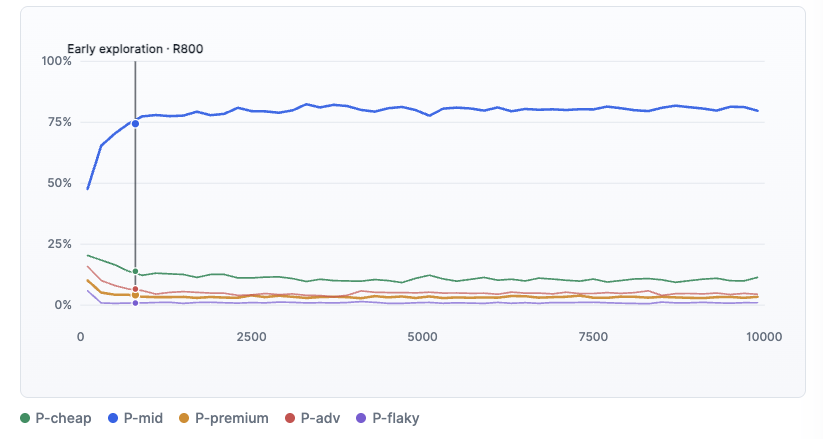
\includegraphics[width=0.32\textwidth]{figures/S1.png}\hfill
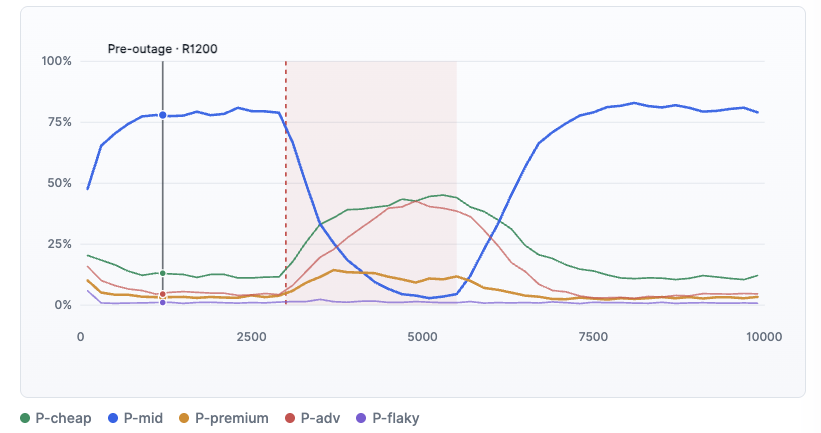
\includegraphics[width=0.32\textwidth]{figures/S2.png}\hfill
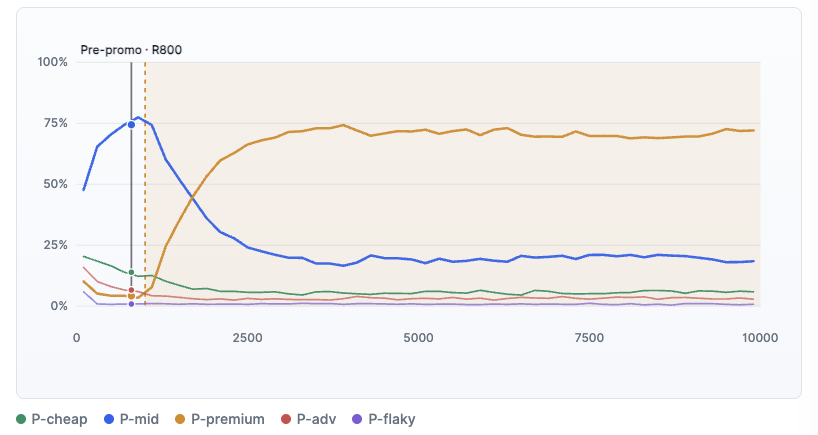
\includegraphics[width=0.32\textwidth]{figures/S3.png}
\caption{PA-DCT provider-allocation share over rounds (mean over $30$ seeds) in S1 stationary (left), S2 mid outage (middle, outage window shaded; window is rounds $3{,}000$--$5{,}500$), and S3 premium promo (right, post-shock region shaded; shock at round $1{,}000$). In S1 the policy converges to a P-mid-dominated mix after the early-exploration phase. In S2 it migrates spend away from P-mid as failures accumulate during the outage and migrates back once P-mid recovers. In S3 it shifts the bulk of spend to P-premium within a few hundred rounds of the price drop. Allocation to P-flaky remains low; P-adv is discussed separately because its detectability depends on the evaluator bucket.}
\label{fig:learning-curves}
\end{figure}

% Figure: trailing-200 ROI around the S2 outage window for full PA-DCT vs the
% $-D$ ablation (the data is reported numerically in Table~\ref{tab:ablations}).
% Adding a dedicated panel is deferred to the camera-ready version; in the
% submission the numerical AdaptT contrast (1467 vs 2249, a 35\% gap) and the
% per-component analysis below already isolate the discount's contribution.

\paragraph{Headline.}
Table~\ref{tab:main} should be read as an adaptation trade-off, not as a claim that PA-DCT is the stationary best arm. S1 is a cost-of-adaptation sanity check: the reliable fixed mid-tier arm is strongest on cum-PA ($5831$), and PA-DCT trails it by $\approx\!319$ because it still explores and maintains shock-readiness in a market with no drift. In the two non-stationary scenarios, PA-DCT outperforms $4/5$ non-oracle baselines in S2 and $5/5$ in S3 on cum-PA; the remaining S2 comparison against Always-P-cheap is a statistically non-significant tie ($5147$ vs $5164$), while PA-DCT delivers much higher mean quality ($0.761$ vs $0.610$). In S3, the learned cost posterior lets PA-DCT capture the premium price promotion, beating Always-P-mid on cum-PA ($5911$ vs $5831$), ROI ($429$ vs $410$), and mean quality ($0.831$ vs $0.819$), while shifting most post-shock spend to P-premium in Fig.~\ref{fig:learning-curves}.

\paragraph{Per-baseline narrative.}
\textbf{vs Random and Always-P-cheap.} PA-DCT dominates Random on cum-PA and mean quality in all scenarios. Against Always-P-cheap, the trade-off is sharper: the cheap arm posts the highest ROI ($\approx\!1{,}221$) by spending very little, but at $\bar q = 0.610$ it leaves quality on the table. PA-DCT wins on cum-PA in S1/S3 and statistically ties in S2, where the cheap arm sidesteps the P-mid outage by never using P-mid; PA-DCT's value in that tied cell is quality, not raw reward.
\textbf{vs Always-P-mid.} Always-P-mid is the stationary fixed-arm benchmark. PA-DCT loses to it in S1, which exposes the exploration cost of a shock-ready policy. Under the S2 outage, Always-P-mid is directly penalized by the $30\%$ failure rate, whereas PA-DCT migrates spend away from P-mid and wins on cum-PA. Under the S3 promotion, PA-DCT uses realized cost feedback to exploit the newly cheap premium arm and improves over Always-P-mid on all three reported economic axes.
\textbf{vs Always-P-premium.} Always-P-premium has the highest fixed-arm mean quality, but in S1/S2 it exhausts the \$50 wallet near round $5{,}000$ and accumulates large negative payment-aware reward under high wallet pressure. In S3 it no longer bankrupts after the price cut, but the first $1{,}000$ expensive premium calls still leave it far behind PA-DCT on cum-PA and ROI.
\textbf{vs BudgetRule.} BudgetRule's static escalation triggers at fixed wallet thresholds and cannot detect the S3 price promotion. PA-DCT migrates to P-premium at the first measurable AdaptT window after the round-$1{,}000$ shock and accumulates substantially more cum-PA over the remaining $9{,}000$ rounds.

\paragraph{Adversarial-provider detection.}
The same-price provider design exposes evaluator-bounded adversarial detection. PA-DCT suppresses P-flaky quickly because timeout feedback is explicit. P-adv is harder: deterministic buckets such as T1/T2 make its low utility visible earlier, while T3b open-ended judging occasionally accepts fluent-but-wrong answers, slowing avoidance. During the S2 outage, some residual P-adv selection also reflects the policy's search for alternatives to degraded P-mid; we revisit this evaluator limit in \S\ref{sec:discuss}.

\subsection{Ablations: which classical components transfer}
\label{sec:eval-ablations}

We disable each of PA-DCT's four conceptual components in turn---Payment-aware ranking ($-P$), Discount ($-D$), Contextual bucketing ($-C$), Thompson sampling ($-TS$). Full PA-DCT is a robust shock-adaptive design, not a per-scenario tuning of the highest cum-PA mean, so the ablation asks which component is exposed on which metric. We additionally run a diagnostic ablation that isolates the cost-posterior pathway inside payment-awareness ($-C_{\mathrm{post}}$, which pins cost to the spec scalar $\bar c_a$ while leaving wallet-pressure weighting intact). This diagnostic is meaningful only under price drift, so we run it on S3 only. Table~\ref{tab:ablations} reports deltas relative to full PA-DCT.

\begin{table}[t]
\centering
\small
\setlength{\tabcolsep}{3.5pt}
\caption{Component ablation: rows $-P,-D,-C,-TS$ ablate the four conceptual components of PA-DCT; row $-C_{\mathrm{post}}$ is a diagnostic isolation of the cost-posterior pathway inside $P$ (it pins cost to the spec scalar $\bar c_a$ while leaving wallet-pressure weighting intact). cum-PA is reported as mean$\pm$std over $30$ seeds; ROI, $\bar q$, Regret, and AdaptT as means. Bold marks the metric that most clearly exposes each component's empirical role; AdaptT is defined in \S\ref{sec:eval-comparators}. The $-C_{\mathrm{post}}$ ablation is run on S3 only because realized prices match $\bar c_a$ in S1/S2; those cells are marked \texttt{n.r.} (not run) rather than inferred.}
\label{tab:ablations}
\resizebox{\textwidth}{!}{%
\begin{tabular}{l|cccc|cccc|cccc}
\toprule
& \multicolumn{4}{c|}{S1 Stationary} & \multicolumn{4}{c|}{S2 Mid Outage} & \multicolumn{4}{c}{S3 Premium Promo} \\
Variant & cum-PA & ROI & $\bar q$ & Regret & cum-PA & ROI & $\bar q$ & AdaptT & cum-PA & ROI & $\bar q$ & AdaptT \\
\midrule
Full PA-DCT      & $5512\pm 54$  & $378$ & $0.797$ & $1325$ & $5147\pm 80$  & $357$ & $0.761$ & $\mathbf{1467}$ & $5911\pm 51$  & $429$ & $\mathbf{0.831}$ & $\mathbf{200}$  \\
$-P$             & $\mathbf{-1710\pm 588}$ & $111$ & $0.839$ & $8547$ & $\mathbf{-1966\pm 507}$ & $103$ & $0.839$ & $1611$ & $4528\pm 369$ & $351$ & $0.840$ & $200$  \\
$-D$             & $5745\pm 95$  & $412$ & $0.810$ & $1092$ & $5113\pm 125$ & $399$ & $0.745$ & $\mathbf{2249}$ & $5974\pm 93$  & $426$ & $0.838$ & $\mathbf{279}$  \\
$-C$             & $5679\pm 41$  & $390$ & $0.812$ & $1159$ & $5225\pm 66$  & $368$ & $0.761$ & $1176$ & $6024\pm 35$  & $425$ & $0.848$ & $\mathbf{398}$  \\
$-TS$            & $5540\pm \mathbf{458}$ & $535$ & $0.740$ & $1297$ & $5063\pm \mathbf{481}$ & $537$ & $0.687$ & $1125$ & $5663\pm \mathbf{244}$ & $552$ & $0.742$ & $\mathbf{2232}$ \\
$-C_{\mathrm{post}}$ & \texttt{n.r.} & \texttt{n.r.} & \texttt{n.r.} & \texttt{n.r.} & \texttt{n.r.} & \texttt{n.r.} & \texttt{n.r.} & \texttt{n.r.} & $\mathbf{5681\pm 54}$ & $423$ & $\mathbf{0.797}$ & $\infty$ \\
\bottomrule
\end{tabular}%
}
\end{table}

\paragraph{$-P$ (no payment-aware): uniformly costly.}
Removing the budget-pressure weighting forces selection by raw utility, causing the policy to favour high-quality but expensive arms and exhaust the wallet early. Cumulative reward collapses below zero in S1/S2 ($-1{,}710 \pm 588$ and $-1{,}966 \pm 507$) and remains far below full PA-DCT in S3 ($4{,}528 \pm 369$ vs $5{,}911 \pm 51$), where the round-$1{,}000$ price drop partially bails the policy out post-shock. \emph{Conclusion}: payment-awareness is necessary in absolute terms; no other ingredient compensates for ignoring wallet pressure.

\paragraph{$-D$ (no discount, $\gamma=1$): visible on adaptation time.}
With $\gamma = 1$, cumulative reward is not the axis that justifies discounting: $-D$ is slightly higher in S1/S3 and close in S2. Under shocks, however, discounting changes the response speed. In S2, full PA-DCT recovers in $1{,}467$ rounds versus $2{,}249$ for $-D$, a $35\%$ acceleration. In S3 the gap is smaller ($200$ vs $279$ rounds) because the $9{,}000$-round post-shock window is long enough for either variant to converge on the new opportunity. \emph{Conclusion}: discount earns its place specifically on AdaptT; cumulative reward alone would miss this role.

\paragraph{$-C$ (no contextual, $K_b = 1$): scenario-dependent.}
Contextual bucketing is not uniformly beneficial in this benchmark. A single global bucket is faster in S2 ($1{,}176$ vs full $1{,}467$ rounds) because the outage hits all task types uniformly and per-bucket fragmentation slows evidence accumulation. It also attains higher cum-PA means in these finite replay runs. In S3, however, full PA-DCT captures the promotion faster ($200$ vs $398$ rounds) because task-type heterogeneity makes the premium arm especially valuable in hard buckets. \emph{Conclusion}: contextual bucketing is a structural choice for heterogeneous task-provider value, not a free win on every aggregate metric.

\paragraph{$-TS$ (no Thompson sampling, greedy posterior mean): variance and opportunity detection.}
Greedy variants are close to full PA-DCT on S1/S2 cum-PA means but have much higher seed-to-seed standard deviation (full $\approx 50$--$80$; $-TS$ $244$--$481$). In S3 the mean gap is also material ($5{,}663$ vs $5{,}911$), and the greedy variant fails to detect the price shock in $6$ of $30$ seeds (AdaptT $2{,}232$ vs full $200$ among runs that do adapt). \emph{Conclusion}: Thompson sampling makes shock detection routine rather than initialization-dependent; mean cum-PA alone hides the risk.

\paragraph{$-C_{\mathrm{post}}$ (no learned cost posterior, $c$ pinned to $\bar c_a$): isolates the price-shock signal.}
With cost held to the spec scalar, the policy is structurally blind to price drift: the C-posterior never updates, so a price drop cannot show up in the sampled $\hatc{a}{k}$ that feeds the decision rule. We measure this on S3, where P-premium's effective price drops to the mid tier at round $1{,}000$ and the cost-posterior pathway has something to track: $-C_{\mathrm{post}}$ keeps treating P-premium as ten-times-more-expensive than mid for the entire post-shock $9{,}000$-round window, P-premium share never crosses $4\%$ (vs $\approx\!60\%$ for full PA-DCT), $\bar q$ stays at the S1 level $0.797$, and AdaptT is undefined ($\infty$) because the trailing-$200$ ROI never reaches the promotion-capture threshold. The cum-PA gap of $-230$ ($p<10^{-4}$, paired bootstrap, $30$ seeds) is the price-shock-specific value of the dual posterior. We did not run the S1/S2 cells of this ablation: realized prices match $\bar c_a$ throughout in those scenarios, so we expect (but did not measure) coincidence with full PA-DCT---the table's $-C_{\mathrm{post}}$ row marks those cells \texttt{n.r.} rather than inferring values. \emph{Conclusion}: removing the learned cost posterior collapses S3 to the no-shock baseline. The four classical components $(P,D,C,TS)$ together cannot recover this; the cost posterior is the structural commitment that makes price shocks first-class observations rather than configuration metadata.

\paragraph{Why five metrics, not one.}
No single classical bandit metric reveals all of these contributions. Cumulative reward alone misses $-D$'s adaptation-speed role and can make $-C$ look uniformly preferable in this finite benchmark. ROI alone over-rewards $-TS$ (greedy locks onto cheap arms with high $q/\$$ ratio while missing better-quality opportunities). AdaptT without cumulative reward would miss $-P$'s collapse in S1/S2. Mean quality $\bar q$ exposes $-C_{\mathrm{post}}$'s failure to migrate to P-premium under the S3 promo (where it stays at the S1 quality level, $0.797$) even though its cum-PA gap is moderate. Regret to the Oracle isolates the cost of $-P$ in the stationary regime where AdaptT is undefined. The five metrics together expose each component on the axis where it matters; this is the multi-metric evaluation framework we recommend for future work in this regime.

\section{Discussion and Limitations}
\label{sec:discuss}

% TODO: ~0.5 page (paper_outline.md §7).
%
% Beats (kept short — limitations honest, future work concrete):
% 1. Pre-payment vs. post-selection. \padct{} sits before the HTTP request;
%    A402 and similar handle post-selection atomicity. Complementary.
% 2. Dataset fidelity. Pre-generated responses freeze model behavior at
%    pregen time. Real markets evolve; the discount γ partially mitigates
%    stale priors. Live deployment would need periodic re-generation.
% 3. Evaluator-bounded P-adv detection. On open-ended T3b, the LLM judge
%    sometimes accepts fluent-but-wrong answers; \padct{}'s detection of
%    P-adv lags accordingly. Stronger evaluators would tighten the gap.
% 4. Single-agent scope. Multi-agent dynamics, auctions, federated learning
%    across agents — out of scope; future work.
% 5. Uniform task-type ordering assumed. The encoder does not stratify
%    provider quality by task type beyond the contextual bucket. Adequate
%    for our calibration where providers differ primarily by tier.
% 6. Future directions: drift detection, online safeguards, real-deployment
%    A/B evidence.

\section{Conclusion}
\label{sec:conclusion}

We formalized \emph{agent-native bandits}: budget-aware, non-stationary, contextual decision-making in programmable micropayment markets where the bandit is the autonomous buyer itself, not a human-operated routing service. The central claim that follows from this formalization is that autonomous payment is not only a settlement problem; it is an online economic decision problem in which the buyer must learn both service quality and price simultaneously, and the buyer-optimal policy is therefore wallet-, context-, and shock-aware---never any fixed-arm strategy. We proposed \emph{402Pilot}, a protocol-agnostic buyer-side decision layer that separates this decision from settlement and runs above x402 (or AP2, A2A--x402, A402, any future quote-and-pay protocol). Inside the layer we proposed \emph{PA-DCT}, a payment-aware Thompson-sampling rule built from four conceptual components (payment-awareness, discount, contextual bucketing, Thompson sampling), where payment-awareness is grounded in a \emph{learned cost posterior} that lets a single policy detect price shocks and quality shocks symmetrically.

On 402Pilot-Bench---a reproducible benchmark of $823$ tasks $\times$ $5$ providers (including same-price adversarial and flaky variants) $\times$ $3$ calibrated market scenarios with $30$ seeds and $10{,}000$ rounds per cell---PA-DCT recovers from a mid-tier outage $35\%$ faster than its no-discount variant, adapts within $\approx\!200$ rounds to a premium price promotion, and Pareto-dominates every fixed-arm baseline on (cum-PA, $\bar q$) in both non-stationary scenarios while paying only a small honest exploration cost when the market is stationary. The four-component ablation, plus a diagnostic isolation of the cost-posterior pathway, shows each ingredient is exposed on a different axis: payment-awareness on cumulative reward (uniformly necessary), discount on adaptation time, contextual bucketing selectively when shock structure is task-type heterogeneous, Thompson sampling on seed variance and shock-detection reliability, and the cost posterior on the price-shock channel of S3. No single classical metric reveals all of these; this motivates the five-metric framework (cum-PA, ROI, $\bar q$, regret, AdaptT) we recommend for the regime.

Code, the frozen pre-generated dataset, the scenario sweeps, and the evaluation harness are released as the artifact accompanying this paper (URL withheld during anonymous review; an anonymized snapshot is included in the supplemental material). We hope the layer interfaces, the algorithm, and the benchmark together invite extension to other agent-native settings beyond the LLM-buyer instance studied here.


% ---------------------------------------------------------------------
\bibliographystyle{plain}
\bibliography{references}

% ---------------------------------------------------------------------
\appendix
\section{Notation}
\label{appendix:notation}

% TODO: port logs/notation.md sections 1-9 as a paper appendix.
% Goal: reviewers find every symbol on a single page.
%
% Sections to include:
%   A.1 Time, arms, contexts (table)
%   A.2 Per-round observations
%   A.3 Reward / utility (with formulas)
%   A.4 Discount
%   A.5 Posteriors (Q + C closed forms)
%   A.6 Decision rule
%   A.7 Scenarios (locked specs)
%   A.8 Metrics
%   A.9 Ablation labels
%
% Use the LaTeX preamble macros already defined in main.tex.


\end{document}
